%%%%%%%%%%%%%%%%%%%%%%%%%%%%%%%%%%%%%%%%%%%%%%%%%%%%%%%%%
%%             东南大学数电实验报告 LaTeX 模板
%%               Experiment 3 Report.tex
%% https://github.com/Teddy-van-Jerry/SEU_Digital_Report
%% ======================================================
%% 版本信息:
%% v1.0 (Nov. 07, 2021)
%% ------------------------------------------------------
%% 模板制作:
%% Teddy van Jerry, (me@teddy-van-jerry.org)
%% * GitHub: https://github.com/Teddy-van-Jerry
%% * Website: https://teddy-van-jerry.org
%% * Blog: https://blog.teddy-van-jerry.org
%% ------------------------------------------------------
%% 使用说明:
%% 1. 编译使用 XeLaTeX 和 Biber
%% 2. 报告基本信息通过修改导言区以 exp 开头的命令
%% 3. 参考文献位于 ref/ref.bib
%% 4. 报告模板依据 MIT License 开源共享
%% ------------------------------------------------------
%% Copyright 2021 (c) Teddy van Jerry
%%
%% Permission is hereby granted, free of charge, to any
%% person obtaining a copy of this software and
%% associated documentation files (the "Software"), to
%% deal in the Software without restriction, including
%% without limitation the rights to use, copy, modify,
%% merge, publish, distribute, sublicense, and/or sell
%% copies of the Software, and to permit persons to whom
%% the Software is furnished to do so, subject to the
%% following conditions:
%%
%% The above copyright notice and this permission notice
%% shall be included in all copies or substantial
%% portions of the Software.
%% 
%% THE SOFTWARE IS PROVIDED "AS IS", WITHOUT WARRANTY OF
%% ANY KIND, EXPRESS OR IMPLIED, INCLUDING BUT NOT
%% LIMITED TO THE WARRANTIES OF MERCHANTABILITY, FITNESS
%% FOR A PARTICULAR PURPOSE AND NONINFRINGEMENT. IN NO
%% EVENT SHALL THE AUTHORS OR COPYRIGHT HOLDERS BE LIABLE
%% FOR ANY CLAIM, DAMAGES OR OTHER LIABILITY, WHETHER IN
%% AN ACTION OF CONTRACT, TORT OR OTHERWISE, ARISING
%% FROM, OUT OF OR IN CONNECTION WITH THE SOFTWARE OR THE
%% USE OR OTHER DEALINGS IN THE SOFTWARE.
%%%%%%%%%%%%%%%%%%%%%%%%%%%%%%%%%%%%%%%%%%%%%%%%%%%%%%%%%%

%% 使用实验报告模板类(字体大小 11pt 约为五号字)
\documentclass[11pt]{SEU-Digital-Report}

%%%%%%%%%%%%%%%%%%%% 报告基本信息 %%%%%%%%%%%%%%%%%%%%
\expno{五} % 实验序号
\expname{计算机系统与指令认识} % 实验名称
\expauthor{赵舞穹} % 姓名
\expID{61520522} % 学号
\expmates{郑瑞琪} % 同组
\expmatesID{61520523} % 学号(同组)
\expmajor{工科试验班} % 专业
\explab{计算机硬件技术} % 实验室
\expdate{2021年11月26日} % 实验日期
\expreportdate{\today} %报告日期
\expgrade{} % 成绩评定
\exptutor{冯熳} % 评阅教师
%%%%%%%%%%%%%%%%%%%%%%%%%%%%%%%%%%%%%%%%%%%%%%%%%%%%

\usepackage{pgfplots}
\pgfplotsset{compat=1.11}
\usepackage[export]{adjustbox} % for figure border

%% 报告正文
\begin{document}
  % 打印封面页
  \exptitlepage

  \tableofcontents
  \newpage

  \section{实验目的}
        
    \begin{enumerate}
        \item 掌握学习通过模拟调试工具软件认识理解计算机基本资源及动态调试程
        序的概念;
        \item 学习掌握计算机命令行操作方法,了解系统调用的概念;
        \item 学习掌握利用 QtSpim 认识和调试Mips 指令,加深指令理解认识;
        \item 了解计算机命令行操作,认识Debug/TD 调试器及X86 指令调试,加深指
        令理解认识.    \cite{guide}
    \end{enumerate}

  \section{实验内容}

    \subsection{计算机系统环境与命令行认识}

      我对于命令行认识相对较多,平时很多工作也都是在控制台操作的.
      我平时使用的操作系统包括了 MacOS,Linux(Ubuntu)和 Windows.    
      在 MacOS 和 Linux 下很多命令是一样的,使用起来感觉就很流畅.
      Windows 下的 CMD 使用不是很熟练,一般使用其 PowerShell.

      新建文件使用 \texttt{touch},修改文件名或者移动 \texttt{mv},删除 \texttt{rm},编辑可以用 \texttt{nano} 或者 \texttt{vim}.    
      控制台运行的效果如图 \ref{fig:console} 所示.

      下面给出我使用 C++ 的方法:我目前直接使用 \texttt{clang++} 编译,而这样实际非常方便,正如下面的代码给出的这样\footnote{
        完整的项目 Dice Simulation 详见我的 GitHub 项目:\url{https://github.com/Teddy-van-Jerry/Dice_Simulation}.
      }.    

      \begin{lstlisting}[title=compile\_rp3d\_clang.sh,language=sh,morekeywords={mkdir,rm}]
#!/bin/sh

# compile_rp3d_clang.sh
#
# Compile ReactPhysics3d into object file using clang++.
# Object files are in folder 'obj'.
# Warnings are disabled.
#
# Teddy van Jerry
# 2021/09/30

# create dirs
mkdir obj
cd obj
mkdir body
mkdir collision
mkdir collision/broadphase
mkdir collision/narrowphase
mkdir collision/narrowphase/GJK
mkdir collision/narrowphase/SAT
mkdir collision/shapes
mkdir constraint
mkdir engine
mkdir systems
mkdir components
mkdir mathematics
mkdir memory
mkdir utils
cd ..

# compile object files
clang++ -w -c "../ext/reactphysics3d/src/body/RigidBody.cpp" -std=c++11 -I ../ext/reactphysics3d/include -o "obj/body/RigidBody.o"
# ...
# Similar commands are omitted here for the sake of space.
# ...

# Compile the HelloWorld example
cd ../src/cpp/HelloWorld

# Create object file of Main.cpp
clang++ -c -std=c++11 Main.cpp -I ../../../ext/reactphysics3d/include -o Main.o

# Create executable
clang++ -std=c++11 \
Main.o \
"../../../usr/obj/body/CollisionBody.o" \
"../../../usr/obj/body/RigidBody.o" \
# ...
# Similar commands are omitted here for the sake of space.
# ...
"../../../usr/obj/utils/DebugRenderer.o" \
-o HelloWorld

# Remove object file
rm Main.o
      \end{lstlisting}

      \begin{figure}[htbp]
        \centering
        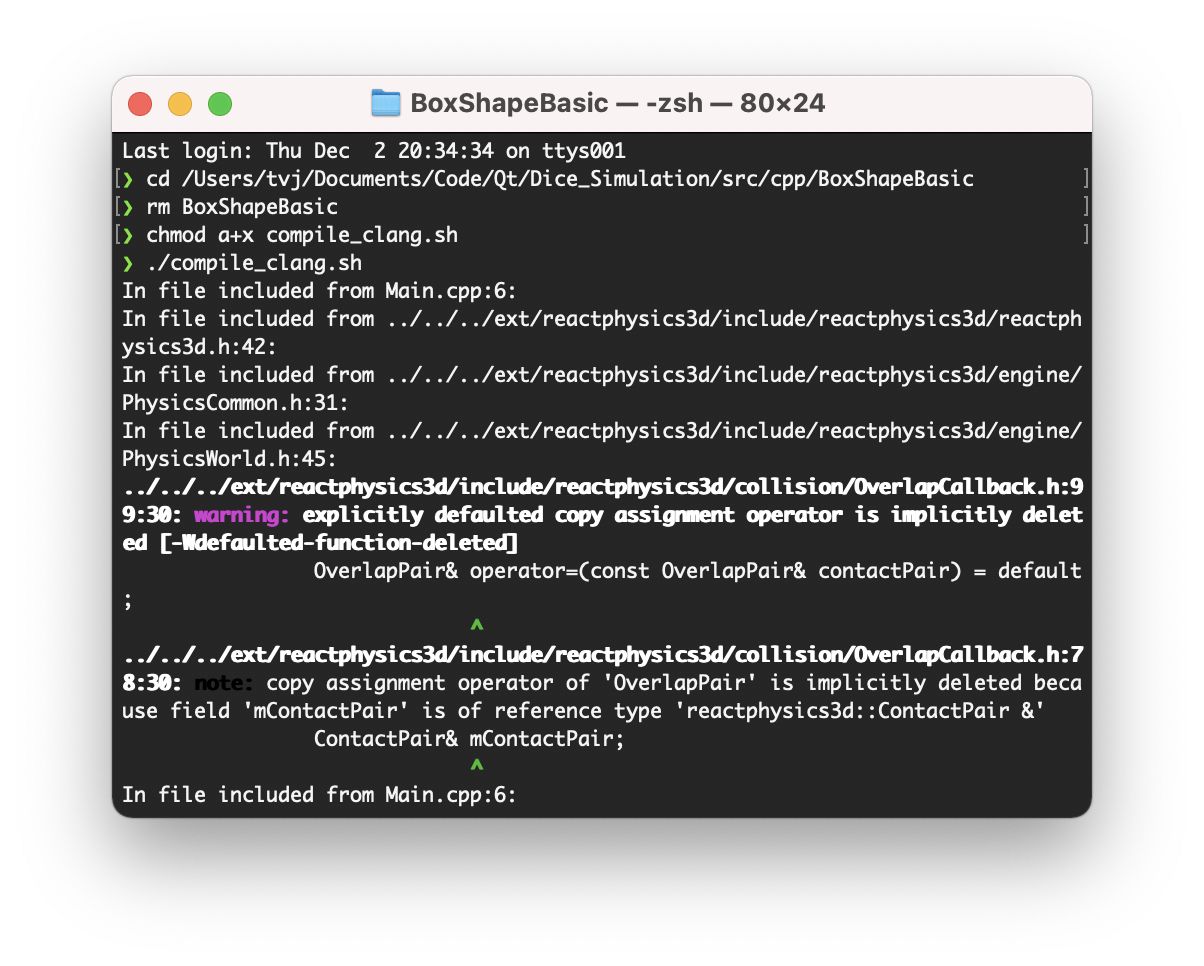
\includegraphics[width=.49\linewidth]{fig/console/1.png}
        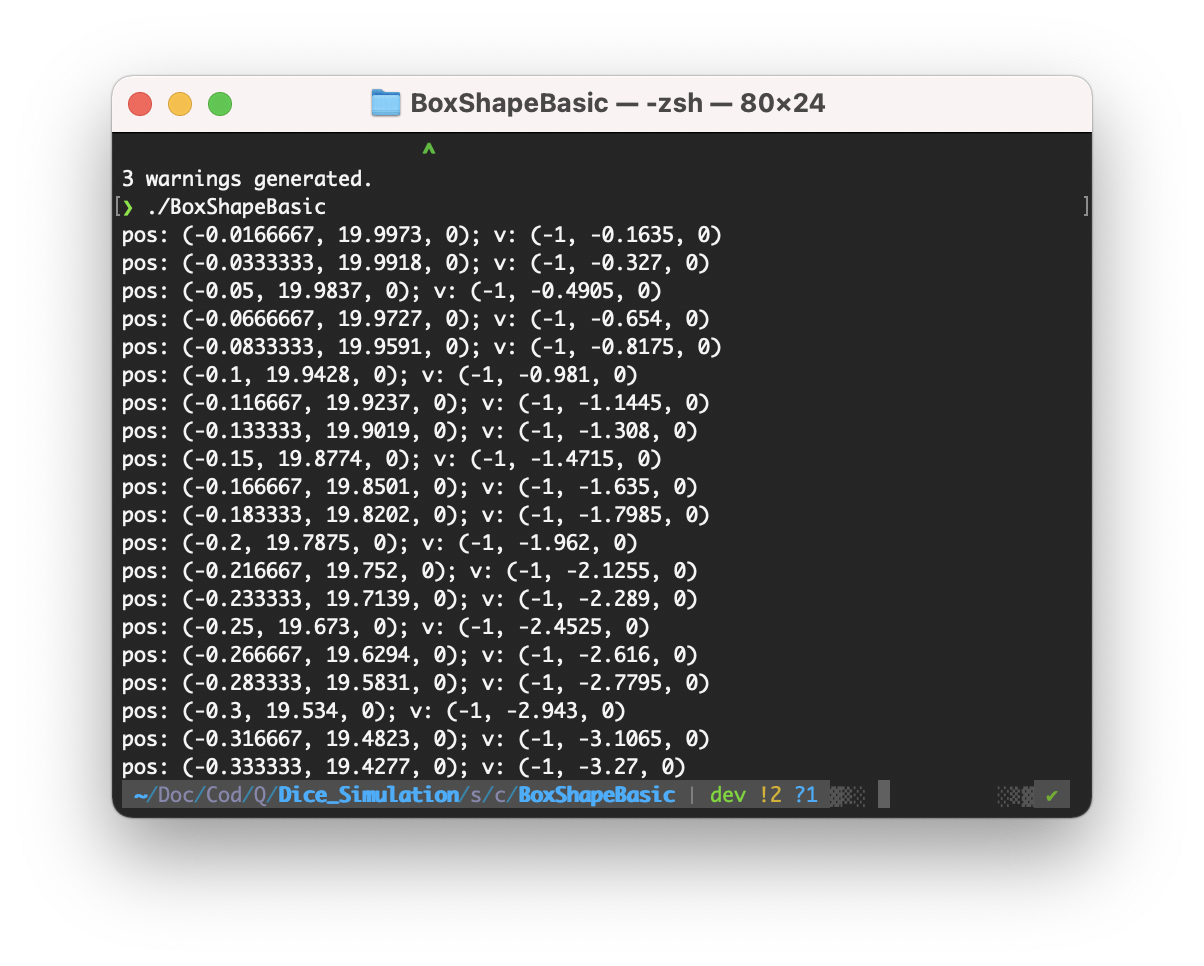
\includegraphics[width=.49\linewidth]{fig/console/2.png}
        \vspace{-5mm}
        \caption{MacOS 控制台编译 C++ 输出}
        \label{fig:console}
      \end{figure}

    \subsection{QtSpim 模拟器与 MIPS 指令验证}

      \subsubsection{Spim 基本测试}

      我在 Ubuntu 平台上,首先安装了无桌面的 Spim 进行测试,命令如下:
    \begin{lstlisting}[language=sh,title={Install Spim on Ubuntu}]
sudo apt install spim # install the command-line version of spim
    \end{lstlisting}

    Terminal 如图~\ref{fig:terminal_spim} 所示.
    首先新建文件 \texttt{spim\_test.m},然后用 Nano 编辑内容,其内容如图~\ref{fig:terminal_nano} 所示.

    \begin{figure}[htbp]
      \centering
      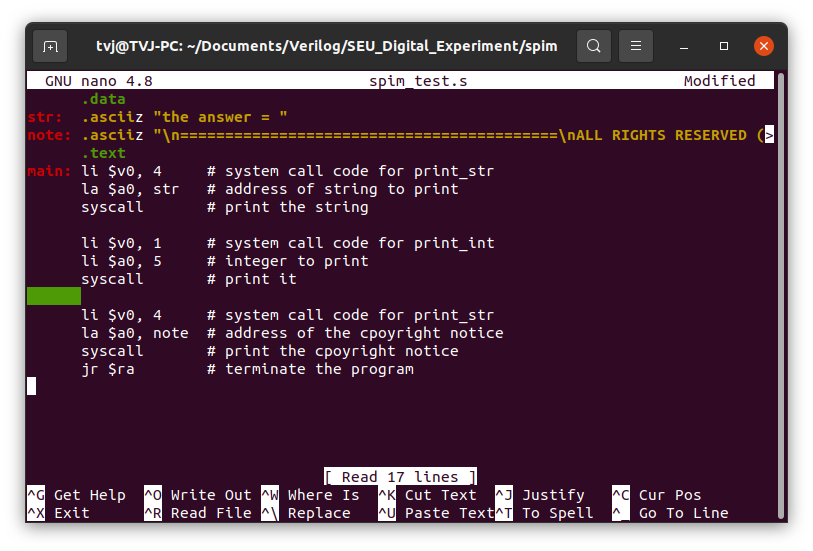
\includegraphics[width=.65\linewidth]{fig/spim/terminal_nano.png}
      \caption{测试代码(Nano 窗口)}
      \label{fig:terminal_nano}
    \end{figure}

    \begin{figure}[htbp]
      \centering
      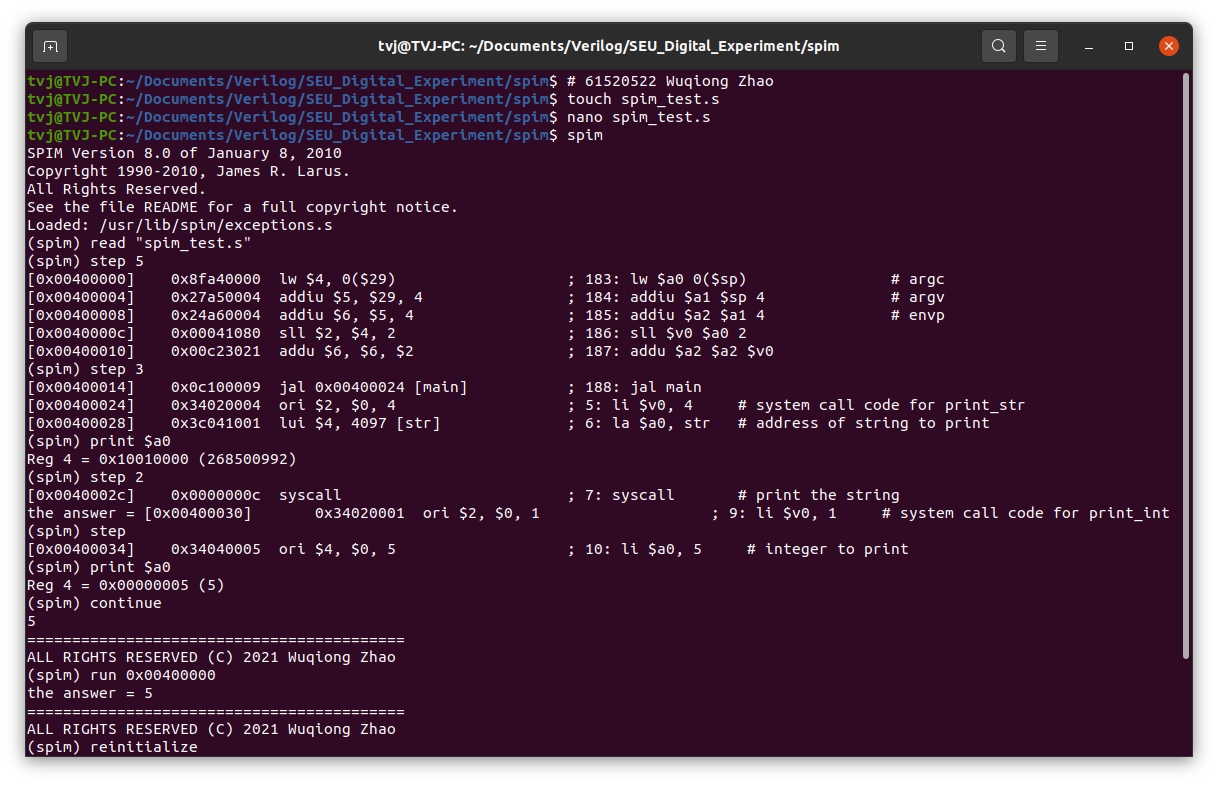
\includegraphics[width=\linewidth]{fig/spim/terminal_spim.png}
      \caption{使用控制台 Spim 直接编译}
      \label{fig:terminal_spim}
    \end{figure}

      然后用 \texttt{spim} 命令进入编译器,首先导入 MIPS 文件(\texttt{read} 或者 \texttt{load}),\texttt{step} 命令单步运行(其后加数字是选择步数),期间可以用 \texttt{print} 命令查看寄存器内变量的值,可以看出 \texttt{\$v0} 对值发生了变化.
      直接继续使用 \texttt{continue} 运行可以看到后续的输出.
      结束之后再使用 \texttt{run} 命令从指定位置开始运行,得到完整的结果.
      再开始其他工作之前需要 \texttt{reinitialize},否则即使是 \texttt{read} 了同一个文件也会出现重复定义现象.

      \begin{note}{报错:{\normalfont\ttfamily attempt to execute non-instruction at 0x0040004c}}{}
        此处最后需要加上 \texttt{jr \$ra},否则 MIPS 程序无法终止.
        \footnote{参考:\url{https://stackoverflow.com/questions/20172655/attempt-to-execute-non-instruction-in-mips-assembler}.}
      \end{note}

      \subsubsection{QtSpim 编译 HelloWorld}

      QtSpim 的界面如图~\ref{fig:qt_spim} 所示,Console 输出如图~\ref{fig:qtspim_console} 所示,其内容与命令行版的 Spim 没有太大区别,只是在显示结果时更加方便.
      Mac 版本的 QtSpim 存在 bug,使用起来还不如直接命令行.

      \begin{figure}[t!]
        \centering
        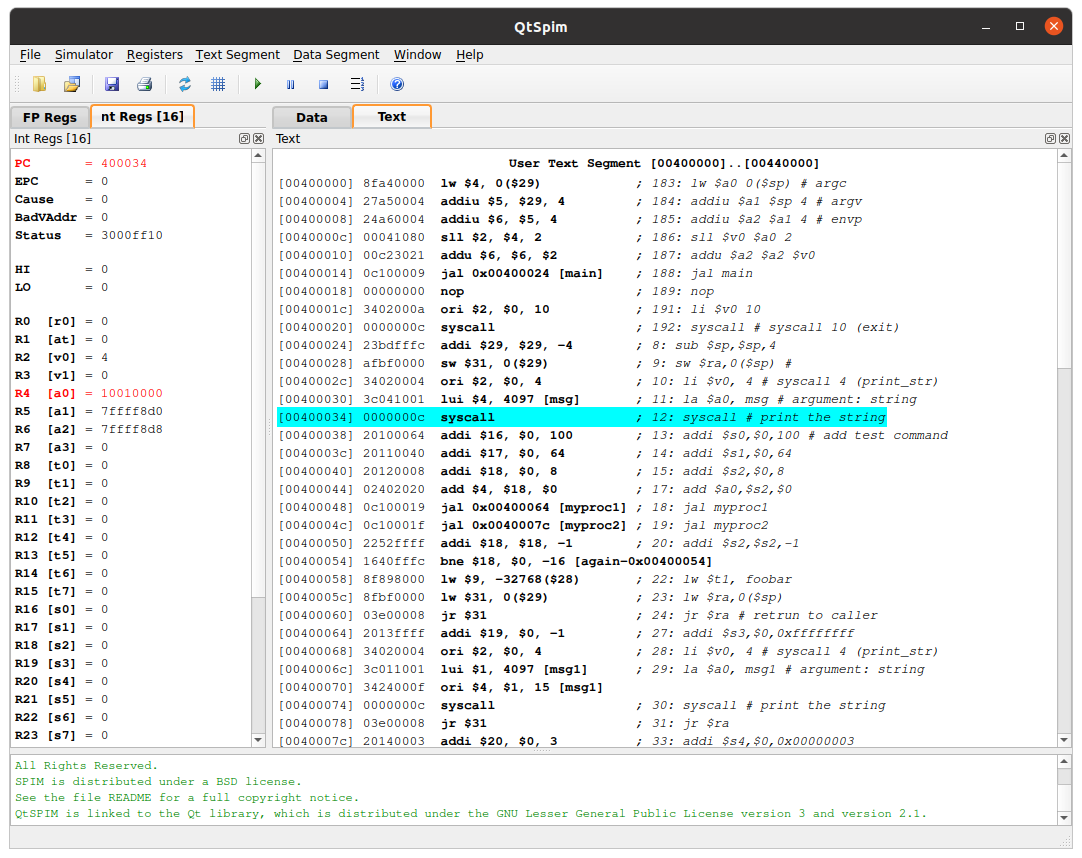
\includegraphics[width=\linewidth]{fig/spim/qt_spim.png}
        \caption{QtSpim 界面(正在单步调试)}
        \label{fig:qt_spim}
      \end{figure}

      \begin{lstlisting}[language=sh,tabsize=4,morekeywords={
        j,la,li,syscall,move,sll,sub,bge,sll,add,sw,addi,jal,ls,subu,jr,lw,bgt,bne
      },title={HelloWorld.s}]
        .data
msg:    .asciiz "Hello World!" # string for display
        .extern foobar 4       # external parameter (exit)

        .text
        .globl main
main:   li $v0, 4       # syscall 4 (print_str)
        la $a0, msg     # argument: string
        syscall         # print the string
        lw $t1, foobar
        
        jr $ra          # return to caller
      \end{lstlisting}

            \begin{lstlisting}[language=sh,tabsize=4,morekeywords={
        j,la,li,syscall,move,sll,sub,bge,sll,add,sw,addi,jal,ls,subu,jr,lw,bgt,bne,lbu,lb,sb
      },title={HelloWorld2.s}]
        .data
msg:    .asciiz "Hello World!\n\n"  # string for display
msg1:   .asciiz "Hello Friend!\n\n" # string for display
        .extern foobar 4            # external parameter (exit)

        .text
        .globl main
main:   sub $sp,$sp,4
        sw $ra,0($sp)   #
        li $v0, 4       # syscall 4 (print_str)
        la $a0, msg     # argument: string
        syscall         # print the string
        addi $s0,$0,100 # add test command
        addi $s1,$0,64
        addi $s2,$0,8
again:
        add $a0,$s2,$0
        jal myproc1
        jal myproc2
        addi $s2,$s2,-1
        bne $s2,$0,again
        lw $t1, foobar
        lw $ra,0($sp)
        jr $ra          # return to caller
myproc1:
        addi $s3,$0,0xffffffff
        li $v0, 4       # syscall 4 (print_str)
        la $a0, msg1    # argument: string
        syscall         # print the string
        jr $ra
myproc2:
        addi $s4,$0,0x00000003
        jr $ra
      \end{lstlisting}

      \begin{lstlisting}[language=sh,tabsize=4,morekeywords={
        j,la,li,syscall,move,sll,sub,bge,sll,add,sw,addi,jal,ls,subu,jr,lw,bgt,bne,lbu,lb,sb
      },title={HelloWorld3.s}]
        .data
msg:    .asciiz "Hello World!\n\n"  # string for display
msg1:   .asciiz "Hello Friend!\n\n" # string for display
        .extern foobar 4            # external parameter (exit)
vb1:    .word   0x12345678
vb2:    .word   0xabcdef12

        .text
        .globl main
main:   sub $sp,$sp,4
        sw $ra,0($sp)   #
        li $v0, 4       # syscall 4 (print_str)
        la $a0, msg     # argument: string
        syscall         # print the string
        la $s4,vb1
        lbu $s5,2($s4)
        la $s6,vb2
        lb $s7,1($s6)
        sb $s5,1($s6)
        sb $s7,2($s4)
        addi $s0,$0,100 # add test command
        addi $s1,$0,64
        addi $s2,$0,8
again:
        add $a0,$s2,$0
        jal myproc1
        jal myproc2
        addi $s2,$s2,-1
        bne $s2,$0,again
        lw $t1, foobar
        lw $ra,0($sp)
        jr $ra          # return to caller
myproc1:
        addi $s3,$0,0xffffffff
        li $v0, 4       # syscall 4 (print_str)
        la $a0, msg1    # argument: string
        syscall         # print the string
        jr $ra
myproc2:
        addi $s4,$0,0x00000003
        jr $ra
        

      \end{lstlisting}

      \begin{figure}[htbp]
        \centering
        \subfloat[HelloWorld]{
          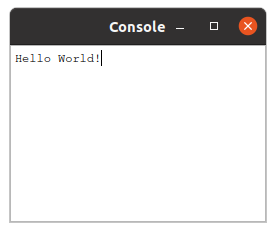
\includegraphics[width=.33\linewidth]{fig/spim/console1.png}
          \label{subfig:console1}
        }
        \subfloat[HelloWorld2]{
          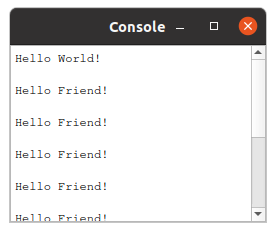
\includegraphics[width=.33\linewidth]{fig/spim/console2.png}
          \label{subfig:console2}
        }
        \subfloat[HelloWorld3]{
          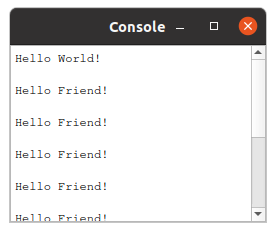
\includegraphics[width=.33\linewidth]{fig/spim/console3.png}
          \label{subfig:console3}
        }
        \caption{HelloWorld 的 Console 输出}
        \label{fig:qtspim_console}
      \end{figure}

      \subsubsection{选择排序的 MIPS 实现}

      使用 MacPort 安装控制台版的 Spim,命令如下:

      \begin{lstlisting}[language=sh,title={Install Spim on MacOS with MacPort}]
sudo port install spim # install the command-line version of spim
      \end{lstlisting}

      通过学习网上的代码,修改相应的内容(因为原来的代码是无法运行的,例如 \texttt{subi} 等命令,与 Spim 的要求不完全匹配),整理设计,得到了如下的代码:

      \begin{lstlisting}[language=sh,tabsize=2,morekeywords={
        j,la,li,syscall,move,sll,sub,bge,sll,add,sw,addi,jal,ls,subu,jr,lw,bgt,bne,lbu,lb,sb
      },title={sort.s}]
        .text
        j	      main	           # Jump to main-routine

        .data
str1:	  .asciiz "Insert the array size: "
str2:	  .asciiz "Insert the array elements, one per line: \n"
str3:	  .asciiz "The sorted array is : \n"
str5:	  .asciiz "\n"

        .text
        .globl	main
main: 
        la	    $a0, str1         # Print of str1
        li	    $v0, 4            #
        syscall	                  #

        li	    $v0, 5            # Get the array size(n) and
        syscall	                  # and put it in $v0
        move    $s2, $v0          # $s2=n
        sll	    $s0, $v0, 2       # $s0=n*4
        sub	    $sp, $sp, $s0     # This instruction creates a stack
                                  # frame large enough to contain
                                  # the array
        la	    $a0, str2         #
        li	    $v0, 4            # Print of str2
        syscall	                  #

        move    $s1, $zero        # i=0

for_get:
        bge	    $s1, $s2, exit_get # if i>=n go to exit_for_get
        sll	    $t0, $s1, 2       # $t0=i*4
        add	    $t1, $t0, $sp     # $t1=$sp+i*4
        li	    $v0, 5            # Get one element of the array
        syscall	                  #
        sw	    $v0, 0($t1)       # The element is stored
                                  # at the address $t1
        addi    $s1, $s1, 1       # i=i+1
        j       for_get

exit_get:
        move    $a0, $sp          # $a0=base address af the array
        move    $a1, $s2          # $a1=size of the array
        jal	    isort             # isort(a,n)
                                  # In this moment the array has been
                                  # sorted and is in the stack frame
        la      $a0, str3         # Print of str3
        li	    $v0, 4            #
        syscall
        move     $s1, $zero       # i=0

for_print:
        bge	    $s1, $s2, exit_print # if i>=n go to exit_print
        sll	    $t0, $s1, 2       # $t0=i*4
        add	    $t1, $sp, $t0     # $t1=address of a[i]
        lw	    $a0, 0($t1)       #
        li	    $v0, 1            # print of the element a[i]
        syscall                   #

        la	    $a0, str5
        li	    $v0, 4
        syscall
        addi    $s1, $s1, 1       # i=i+1
        j       for_print

exit_print:
        add     $sp, $sp, $s0     # elimination of the stack frame
              
        li	    $v0, 10           # EXIT
        syscall
        
# selection_sort
isort:
        addi    $sp, $sp, -20     # save values on stack
        sw      $ra, 0($sp)
        sw      $s0, 4($sp)
        sw      $s1, 8($sp)
        sw      $s2, 12($sp)
        sw      $s3, 16($sp)

        move    $s0, $a0          # base address of the array
        move    $s1, $zero        # i=0

        addi    $t0, $0, 1        # $t0 = 1
        subu    $s2, $a1, $t0     # lenght -1

isort_for:
        bge 	  $s1, $s2, isort_exit # if i >= length-1 -> exit loop
        
        move    $a0, $s0          # base address
        move    $a1, $s1          # i
        move    $a2, $s2          # length - 1
        
        jal	    mini
        move    $s3, $v0          # return value of mini
        
        move    $a0, $s0          # array
        move    $a1, $s1          # i
        move    $a2, $s3          # mini
        
        jal	    swap

        addi	  $s1, $s1, 1       # i += 1
        j	      isort_for         # go back to the beginning of the loop
        
isort_exit:
        lw	    $ra, 0($sp)       # restore values from stack
        lw	    $s0, 4($sp)
        lw	    $s1, 8($sp)
        lw	    $s2, 12($sp)
        lw	    $s3, 16($sp)
        addi	  $sp, $sp, 20      # restore stack pointer
        jr	    $ra               # return


# index_minimum routine
mini:
        move	  $t0, $a0          # base of the array
        move	  $t1, $a1          # mini = first = i
        move	  $t2, $a2          # last
        
        sll	    $t3, $t1, 2       # first * 4
        add	    $t3, $t3, $t0     # index = base array + first * 4
        lw	    $t4, 0($t3)       # min = v[first]
        
        addi	  $t5, $t1, 1       # i = 0

mini_for:
        bgt	    $t5, $t2, mini_end # go to min_end

        sll	    $t6, $t5, 2       # i * 4
        add	    $t6, $t6, $t0     # index = base array + i * 4
        lw	    $t7, 0($t6)       # v[index]

        bge	    $t7, $t4, mini_if_exit # skip the if when v[i] >= min
        
        move    $t1, $t5          # mini = i
        move    $t4, $t7          # min = v[i]

mini_if_exit:
        addi    $t5, $t5, 1       # i += 1
        j 	    mini_for

mini_end:
        move    $v0, $t1          # return mini
        jr	    $ra

# swap routine
swap:
        sll	    $t1, $a1, 2       # i * 4
        add	    $t1, $a0, $t1     # v + i * 4
        
        sll	    $t2, $a2, 2       # j * 4
        add	    $t2, $a0, $t2     # v + j * 4
 
        lw	    $t0, 0($t1)       # v[i]
        lw	    $t3, 0($t2)       # v[j]

        sw	    $t3, 0($t1)       # v[i] = v[j]
        sw	    $t0, 0($t2)       # v[j] = $t0

        jr	    $ra
      \end{lstlisting}

      测试结果如图~\ref{fig:terminal_spim_mac} 所示,成功完成排序.

      \begin{figure}[htbp]
        \centering
        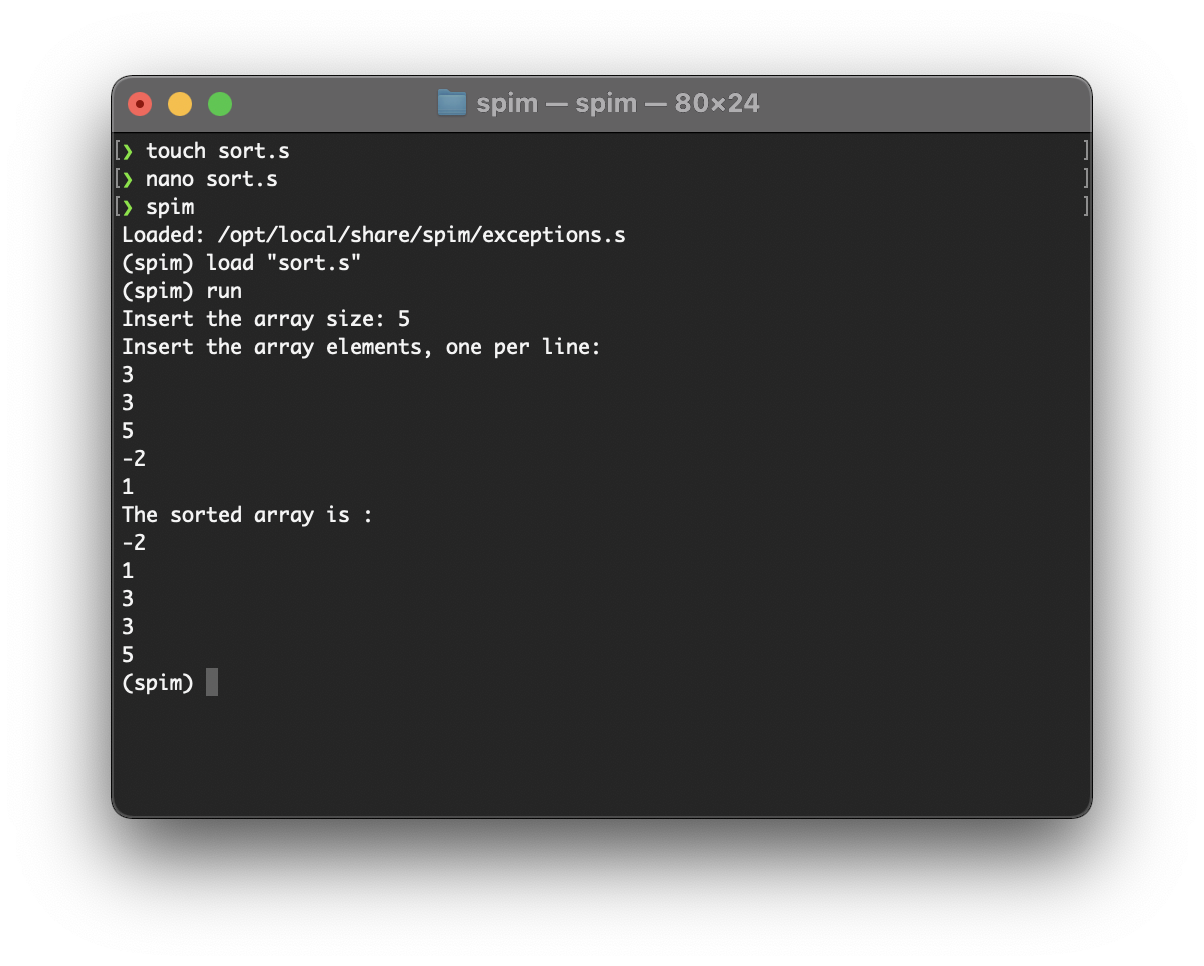
\includegraphics[width=.7\linewidth]{fig/spim/terminal_spim_mac.png}
        \vspace{-5mm}
        \caption{sort.s 输出结果}
        \label{fig:terminal_spim_mac}
      \end{figure}

      \begin{analyze}{MIPS 编写心得}{mips}
          MIPS的学习过程和 Unix、Linux 命令行的学习很像,
          就是一开始觉得十分繁琐,永远也记不下来的命令,
          但是在一定的锻炼之下,有了整体的脉络了解后,
          注重结构性和严谨性(不能像某些提供的代码一样,格式乱七八糟,缩紧不注意,这都是影响代码最后的可读性)才不容易写错.
          汇编写起来要求是高的,因为内存管理需要手动操作
          C/C++ 用起来也相对较难是因为指针的封装也没有摆脱内存管理的工作(其实 C++有一定办法回避,例如引用和使用 std 标准库),对个人的提升是很高的.
      \end{analyze}

    \newpage

    \subsection{在线编译 MIPS}

    我将 \href{https://rivoire.cs.sonoma.edu/cs351/wemips/}{WeMips} 的代码 fork 到了我自己新搭建的网站 \url{https://mips.teddy-van-jerry.org},经过测试效果很好,网页如图~\ref{fig:mips_online} 所示.

    \begin{figure}[htbp]
      \centering
      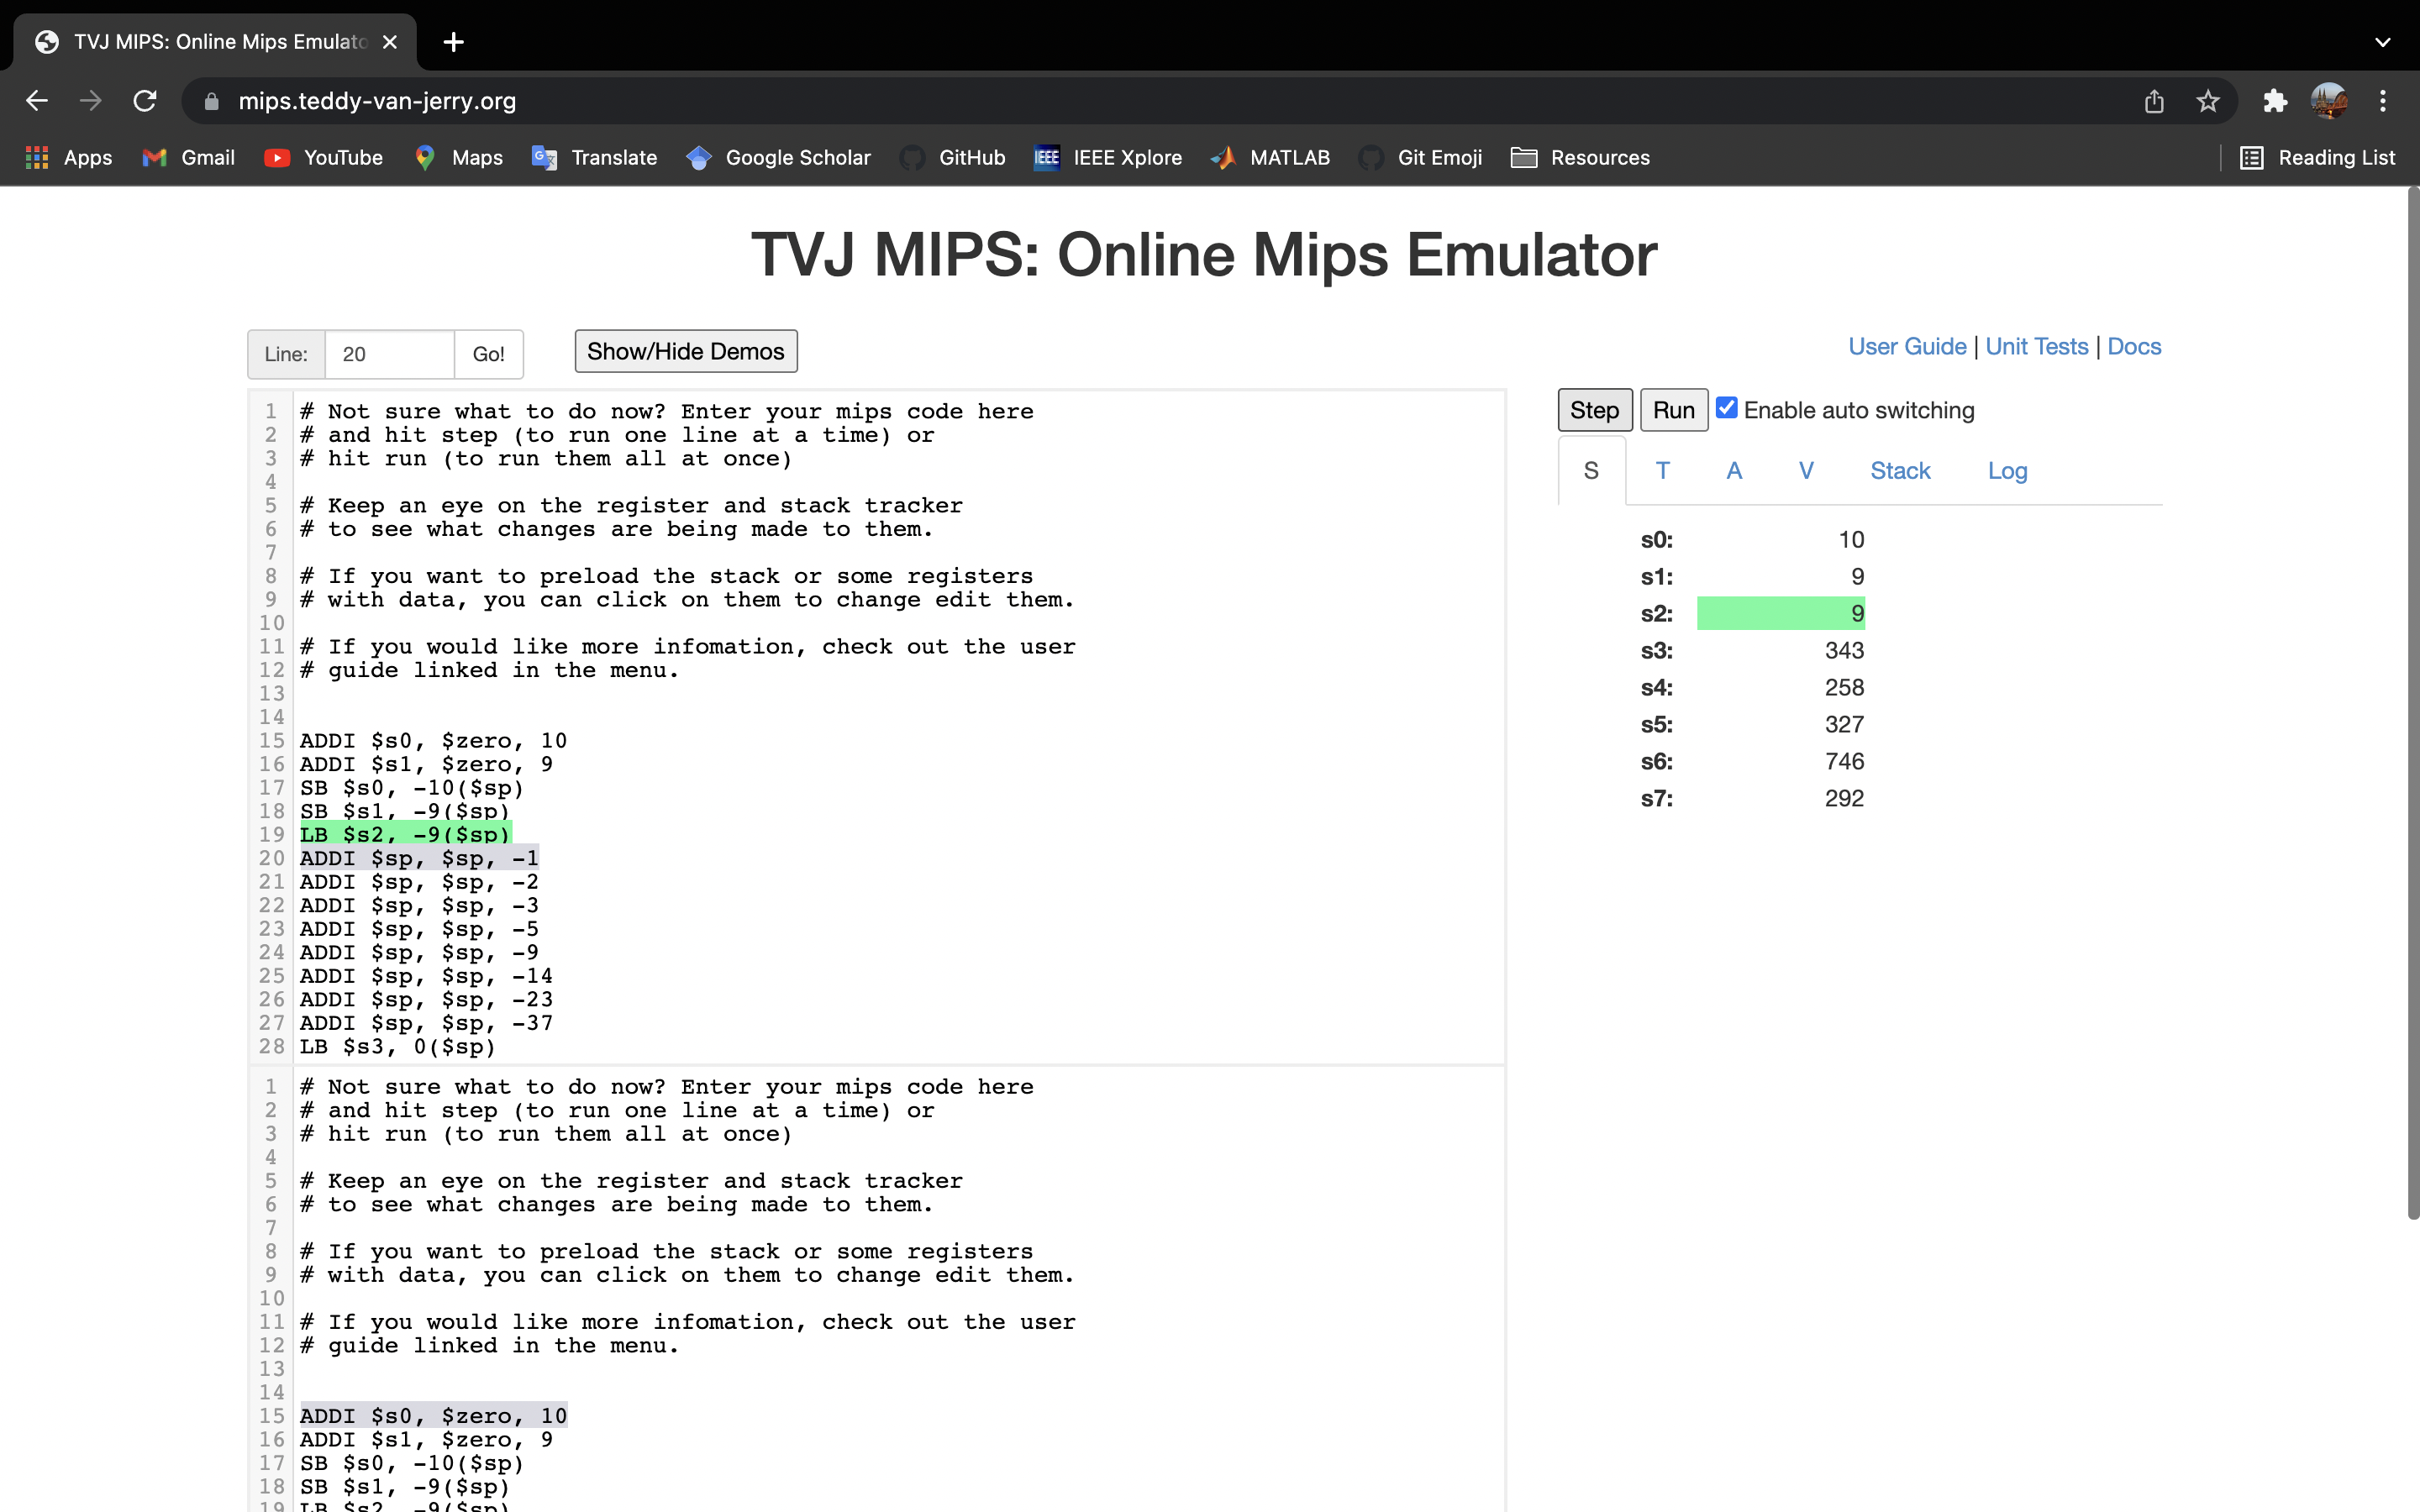
\includegraphics[width=\linewidth,frame]{fig/mips_online.png}
      \caption{TVJ MIPS 在线 MIPS 编译}
      \label{fig:mips_online}
    \end{figure}
      

    \subsection{通过 DOSBox 了解X86指令}

      DOSBox 的实验我在 MacOS 上完成,指导书\cite{guide} 附带的 \texttt{debug.exe} 无法运行,我下载了 \texttt{com} 版本的文件\footnote{资源:\url{https://www.japheth.de/Download/Debug/DEBUG125.zip},包括源代码和 \texttt{com} 文件.},在 MacOS 上使用顺利.

      \newpage

      图~\ref{fig:dos_mount} 为配置 DOSBox 的虚拟挂载路径.
      取消 mount 需要使用命令 \texttt{mount -u <PATH>}.
      \begin{figure}[h!]
        \centering
        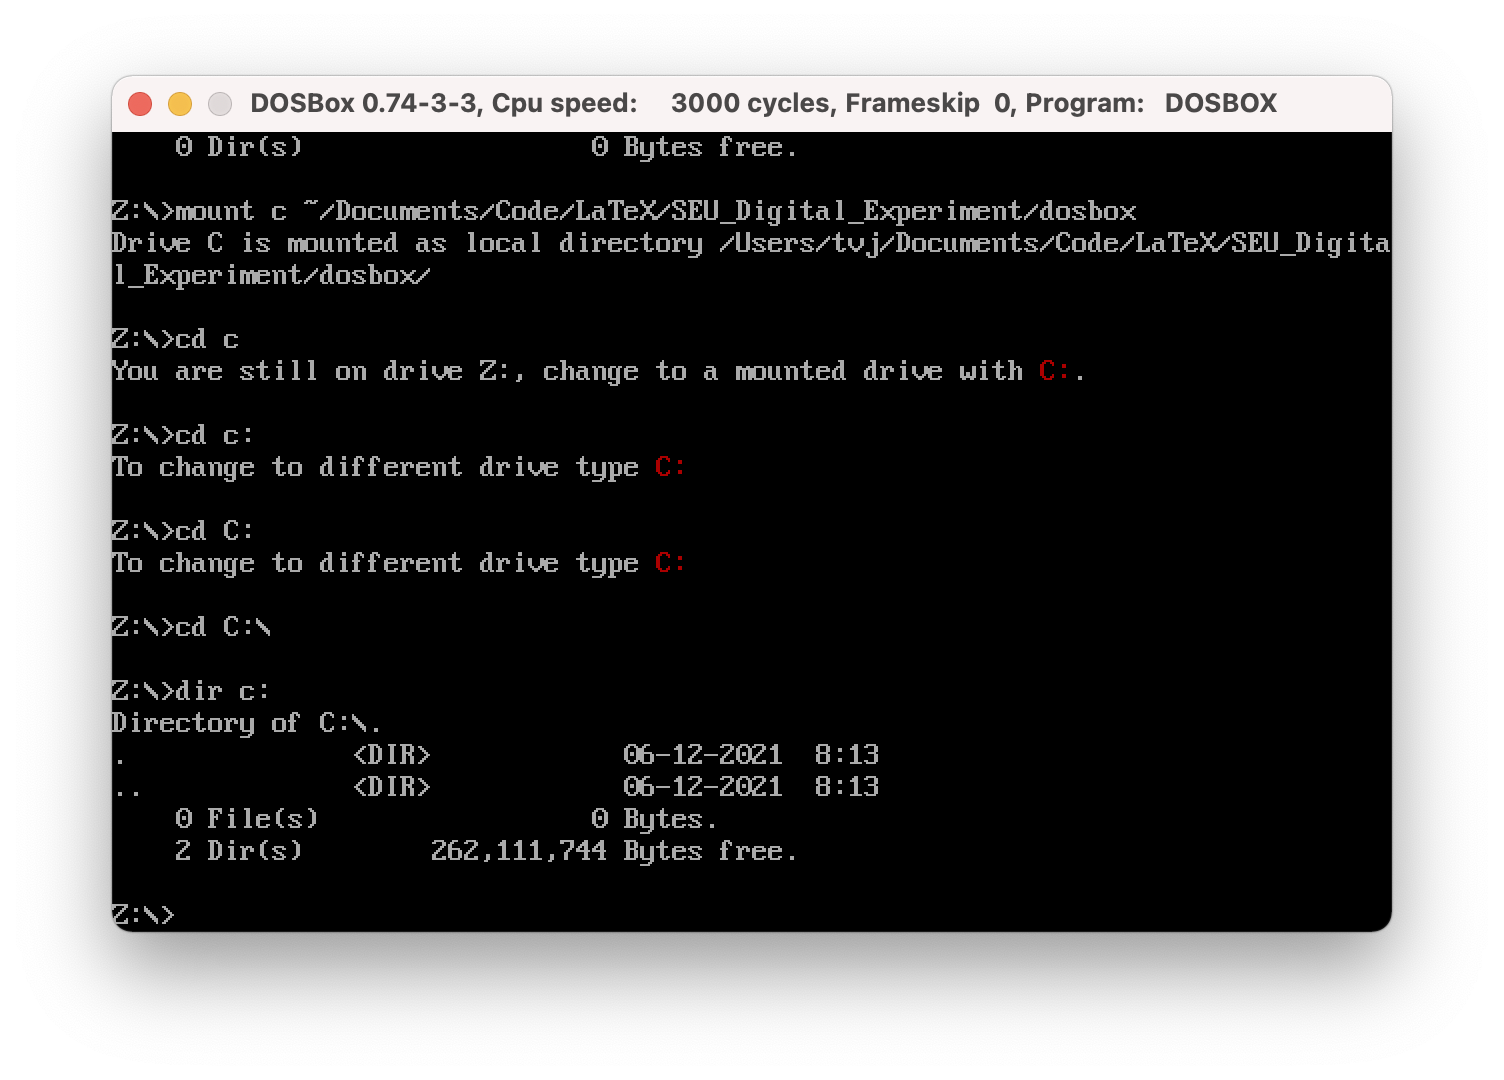
\includegraphics[width=.8\linewidth]{fig/dosbox/mount.png}
        \vspace{-5mm}
        \caption{DOSBox -- mount}
        \label{fig:dos_mount}
      \end{figure}

      %\newpage

      图~\ref{fig:dos_dir} 为通过 \texttt{dir} 命令查看文件夹下的文件和文件夹.
      \begin{figure}[h!]
        \centering
        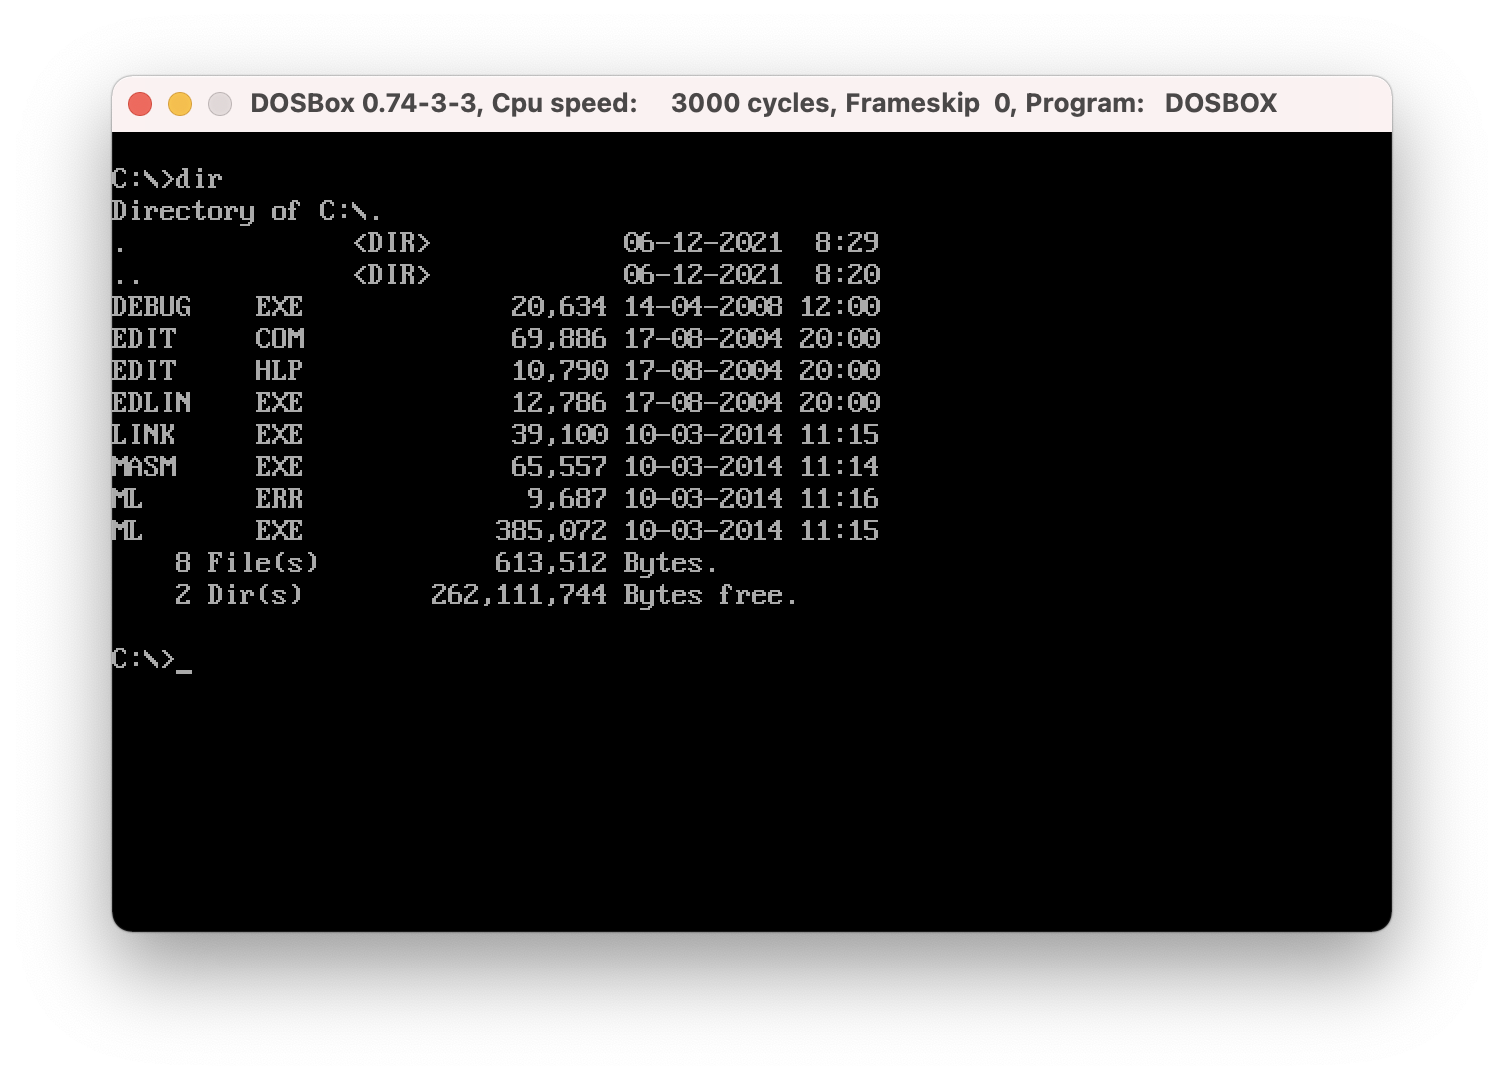
\includegraphics[width=.8\linewidth]{fig/dosbox/dir.png}
        \vspace{-5mm}
        \caption{DOSBox -- dir}
        \label{fig:dos_dir}
      \end{figure}
      
      \newpage

      图~\ref{fig:dos_edit} 使用 \texttt{edit.com} 编辑 \texttt{test1.asm},测试基本的 x86 命令.
      \begin{figure}[htbp]
        \centering
        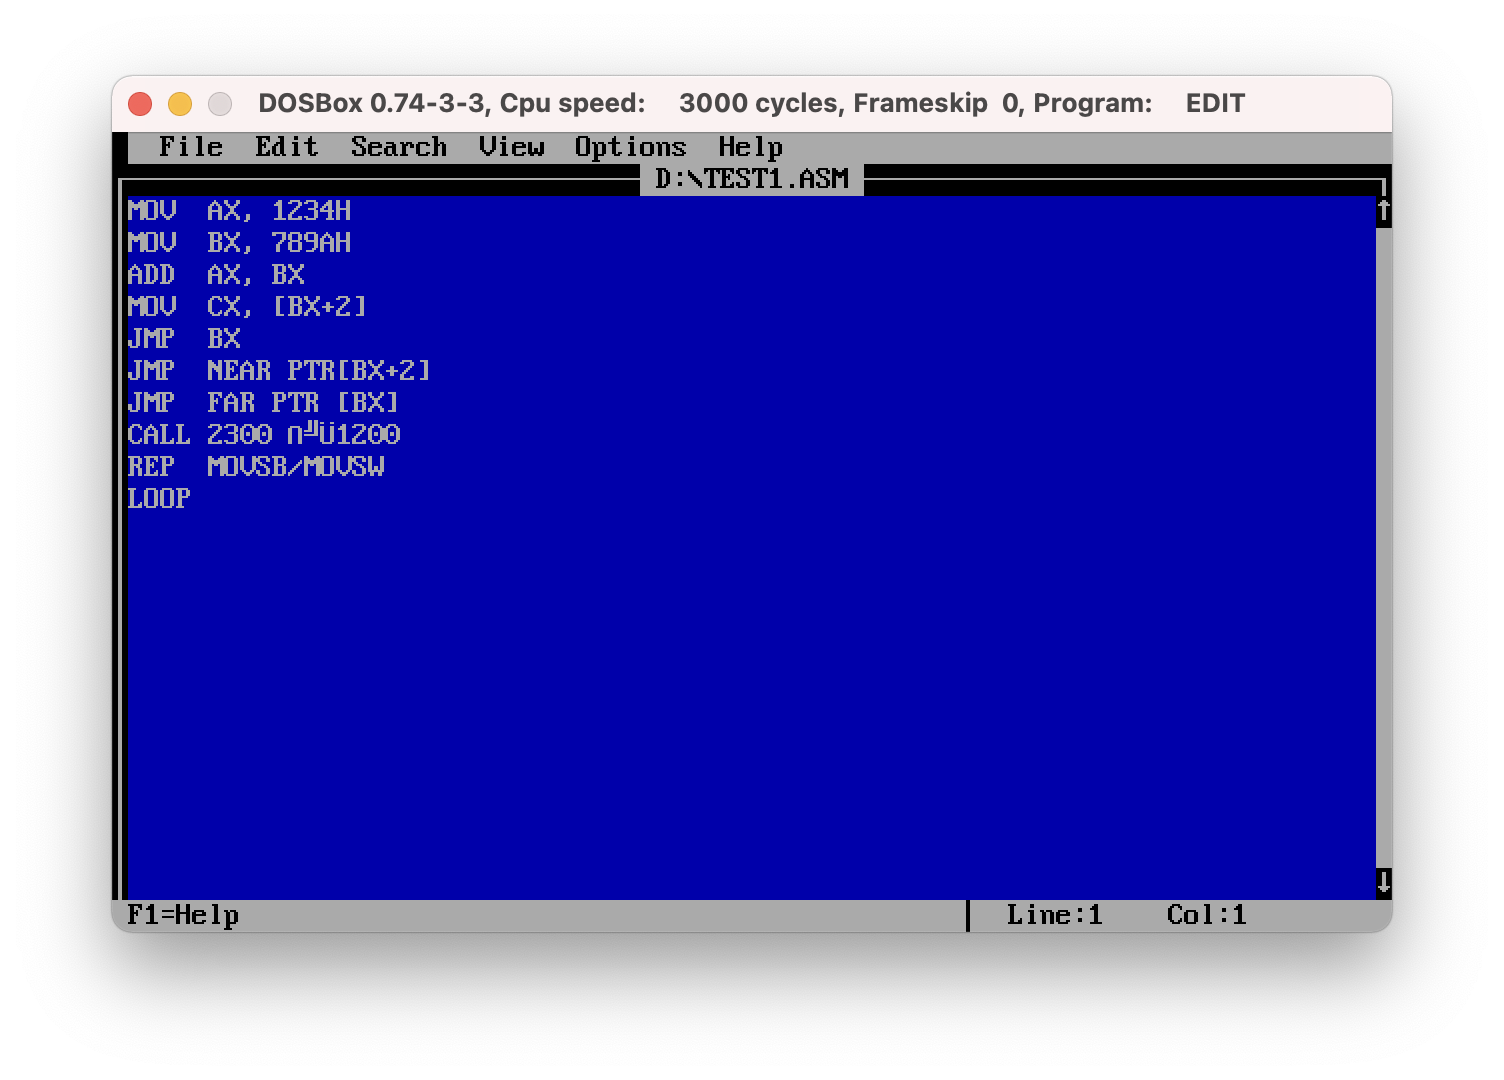
\includegraphics[width=.8\linewidth]{fig/dosbox/edit.png}
        \vspace{-5mm}
        \caption{DOSBox -- edit}
        \label{fig:dos_edit}
      \end{figure}

      %\newpage

      图~\ref{fig:dos_debug} 用 \texttt{debug.com} 运行了刚刚编辑的汇编代码,效果不错.
      \begin{figure}[h!]
        \centering
        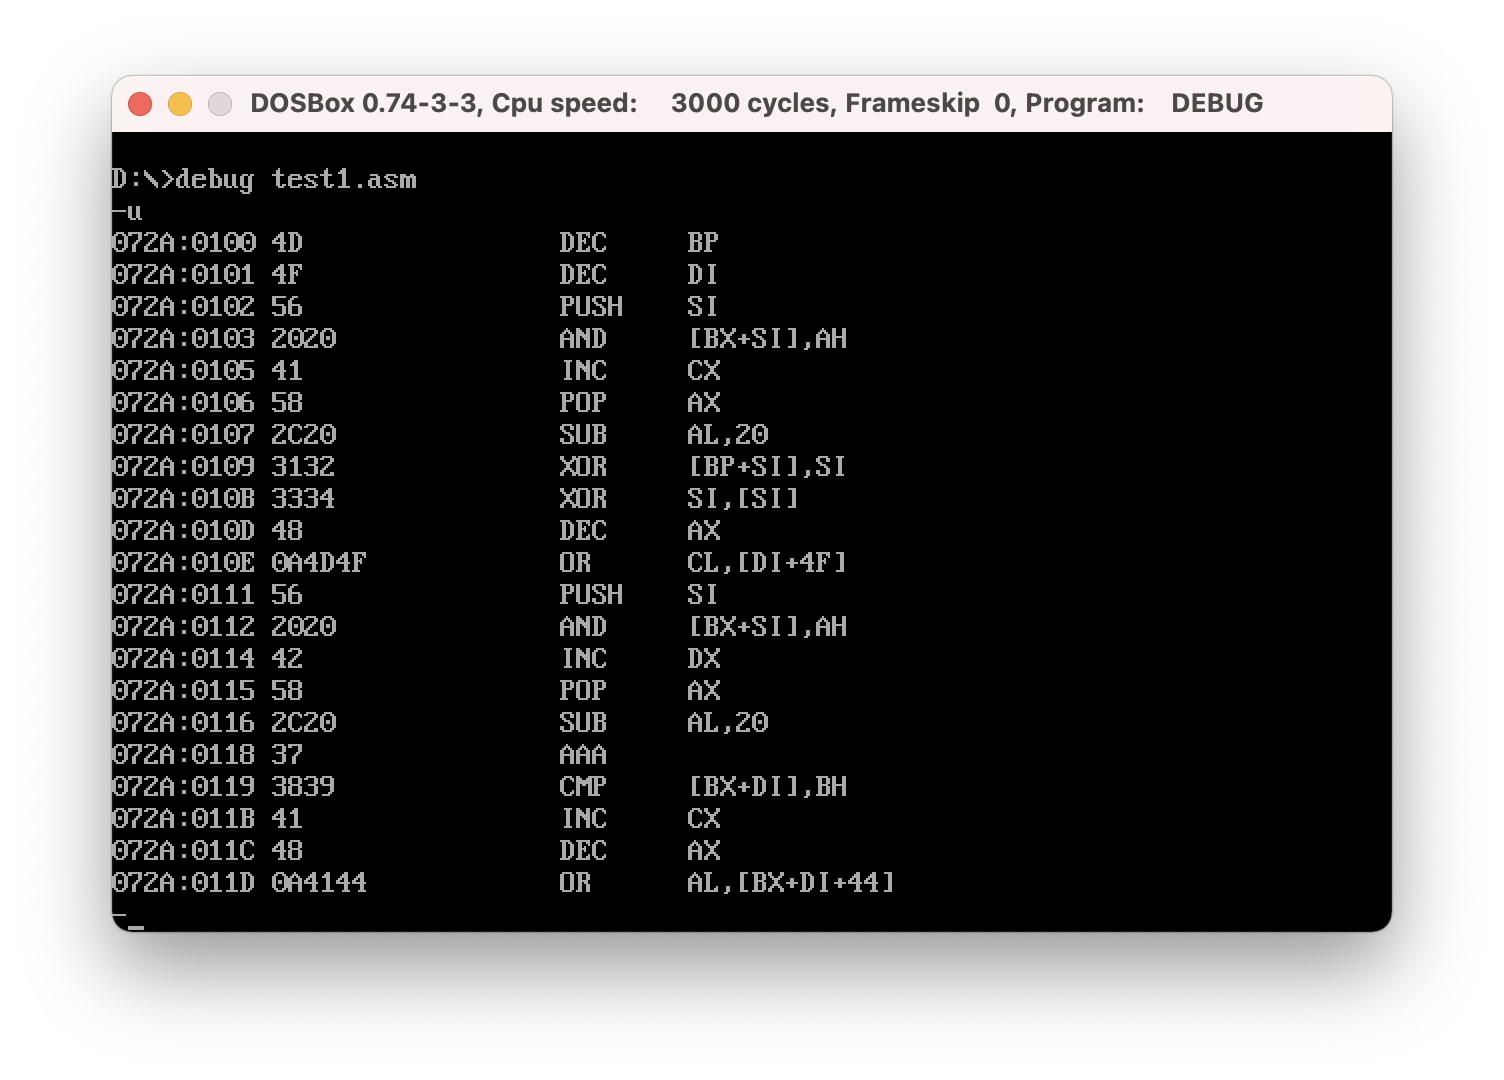
\includegraphics[width=.8\linewidth]{fig/dosbox/debug.png}
        \vspace{-5mm}
        \caption{DOSBox -- debug}
        \label{fig:dos_debug}
      \end{figure}

      \newpage

      图~\ref{fig:dos_speaker} 真的成功让我的 Mac 持续发出固定频率的声音,验证了 DOSBox 在 Mac 上适配性较好.(这么古老的软件居然可以挺让我震惊的.)
      \begin{figure}[h!]
        \centering
        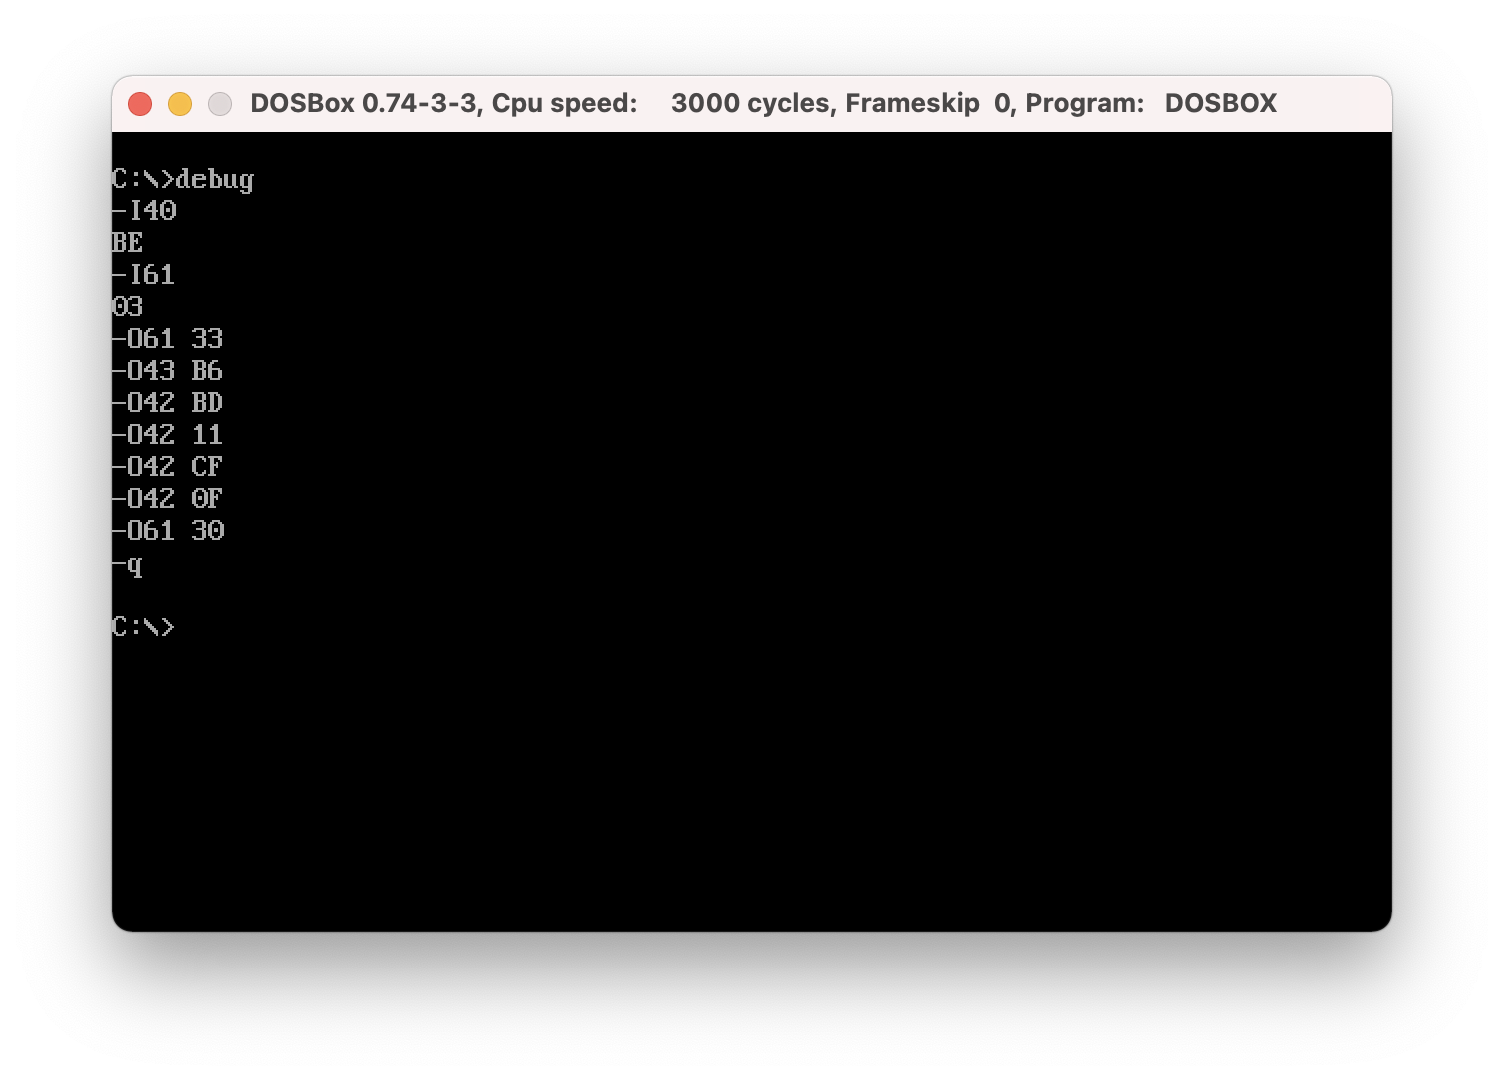
\includegraphics[width=.8\linewidth]{fig/dosbox/speaker.png}
        \vspace{-5mm}
        \caption{DOSBox -- debug(扬声器)}
        \label{fig:dos_speaker}
      \end{figure}

      \begin{analyze}{DOSBox 使用心得}{dosbox}
        有的时候使用这种古老的东西很有那种味道,
        就像我现在比较喜欢用命令行做一些事情一样.
        能够看到古董软件在现代平台上正常运行真实感到不错呢.
      \end{analyze}

  \section{实验创新与提高}

    \begin{itemize}
      \item 多平台使用 QtSpim(Windows,Linux,MacOS),并且使用了命令行版的 Spim;
      \item 编写排序算法,对于汇编的整体架构和使用有了更为深入的了解;
      \item 在自己的网站上搭建了 MIPS 编译器;
      \item DOSBox 中积极解决在 MacOS 上运行的问题,并操作了如 \texttt{mount -u} 等命令.
    \end{itemize}

    

  \section{实验总结}

    关于 MIPS 的总结详见结果分析~\ref{ana:mips},关于 DOSBox 的总结详见结果分析~\ref{ana:dosbox}.
    总体来说,由于我平时有一些命令行的相关了解,也在 Unix,Linux平台上做一些工作,整体的实验比较顺利且有趣.
    这次实验也将更广阔更底层的东西展示给了我,拓展了我的视野.

    \begin{device}{}{devices}
      \begin{itemize}
        \item QtSpim 9.1.21/22
        \item Spim 8.0 (For Ubuntu), Spim 9.1.22 (For MacOS) {\kaishu\color{gray}(无桌面版本)}
        \item DOSBox 0.74-3-3
        \item Ubuntu 20 (X86\_64) / Windows 11 (X86\_64) / MacOS Big Sur (M1 chip){\kaishu\color{gray}(QtSpim 实验于 Ubuntu 和 MacOS 上完成,DOSBox 于 MacOS 上完成)}
        \item Debian GNU/Linux 10 x86\_64 {\kaishu\color{gray}(TVJ MIPS 的服务器)}
      \end{itemize}
    \end{device}
    

    % 打印参考文献
    \addcontentsline{toc}{section}{参考文献}
    \printbibliography[sorting=none]

    % \newpage
    \addcontentsline{toc}{section}{附录 A:实验报告 \LaTeX 模板}
    \section*{附录 A:实验报告 \LaTeX 模板}

        实验报告使用自己编写的 \LaTeX 模板(\texttt{SEU-Digital-Report.cls}),
        在基本适配 Microsoft Word 版报告的格式要求之外,
        增加了更多的功能,使得报告看起来更加优雅多彩.

        后续升级后,报告模板将于 \url{https://github.com/Teddy-van-Jerry/TVJ-Digital-Report} 基于 MIT License 开源共享.

        编译需要使用 \texttt{XeLaTeX + Biber},封面页修改如下内容即可.
        \begin{lstlisting}[
          language=tex,
          morekeywords={
            expno,
            expname,
            expauthor,
            expID,
            expmates,
            expmatesID,
            expmajor,
            explab,
            expdate,
            expreportdate,
            expgrade,
            exptutor,
            today
          }
        ]
%% 使用实验报告模板类(字体大小 11pt 约为五号字)
\documentclass[11pt]{SEU-Digital-Report}

%%%%%%%%%%%%%%%%%%%% 报告基本信息 %%%%%%%%%%%%%%%%%%%%
\expno{五} % 实验序号
\expname{计算机系统与指令认识} % 实验名称
\expauthor{赵舞穹} % 姓名
\expID{61520522} % 学号
\expmates{郑瑞琪} % 同组
\expmatesID{61520523} % 学号(同组)
\expmajor{工科试验班} % 专业
\explab{计算机硬件技术} % 实验室
\expdate{2021年11月26日} % 实验日期
\expreportdate{\today} %报告日期
\expgrade{} % 成绩评定
\exptutor{冯熳} % 评阅教师
%%%%%%%%%%%%%%%%%%%%%%%%%%%%%%%%%%%%%%%%%%%%%%%%%%%%
        \end{lstlisting}

    \addcontentsline{toc}{section}{附录 B:程序真伪判别}
    \section*{附录 B:程序真伪判别}

    \begin{enumerate}
      \item QtSpim 我在报告中使用 Ubuntu 20(GNOME桌面) 和 MacOS Big Sur,窗口非常具有标志性;
      \item Ubuntu 的 Terminal 我加有注释 \texttt{\# 61520522 Wuqiong Zhao} 和 \texttt{ALL RIGHTS RESERVED (C) 2021 Wuqiong Zhao};
      \item DOSBox 使用 MacOS,并且其中的文件日期 \texttt{06-12-2021} 即报告撰写日期.
    \end{enumerate}

\end{document}
